\documentclass{article}
\usepackage{graphicx,subcaption,amsmath,amssymb,amsthm}
\usepackage[margin=2.5cm]{geometry}
\linespread{1.6}
\begin{document}
\section{Single Variable Scenarios}
\begin{figure}
\centering
\begin{subfigure}{0.45\textwidth}
\centering
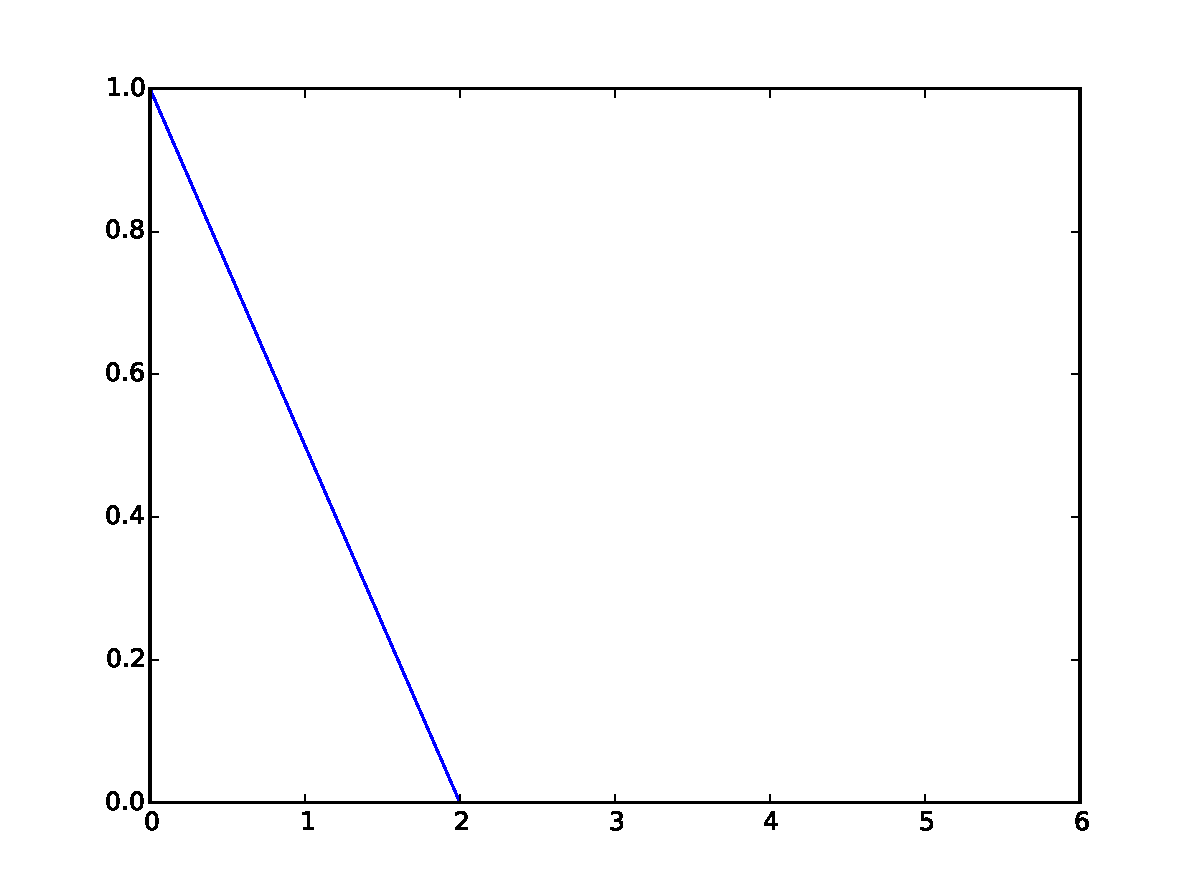
\includegraphics[width=\textwidth]{basis_1.pdf}
\end{subfigure}
\begin{subfigure}{0.45\textwidth}
\centering
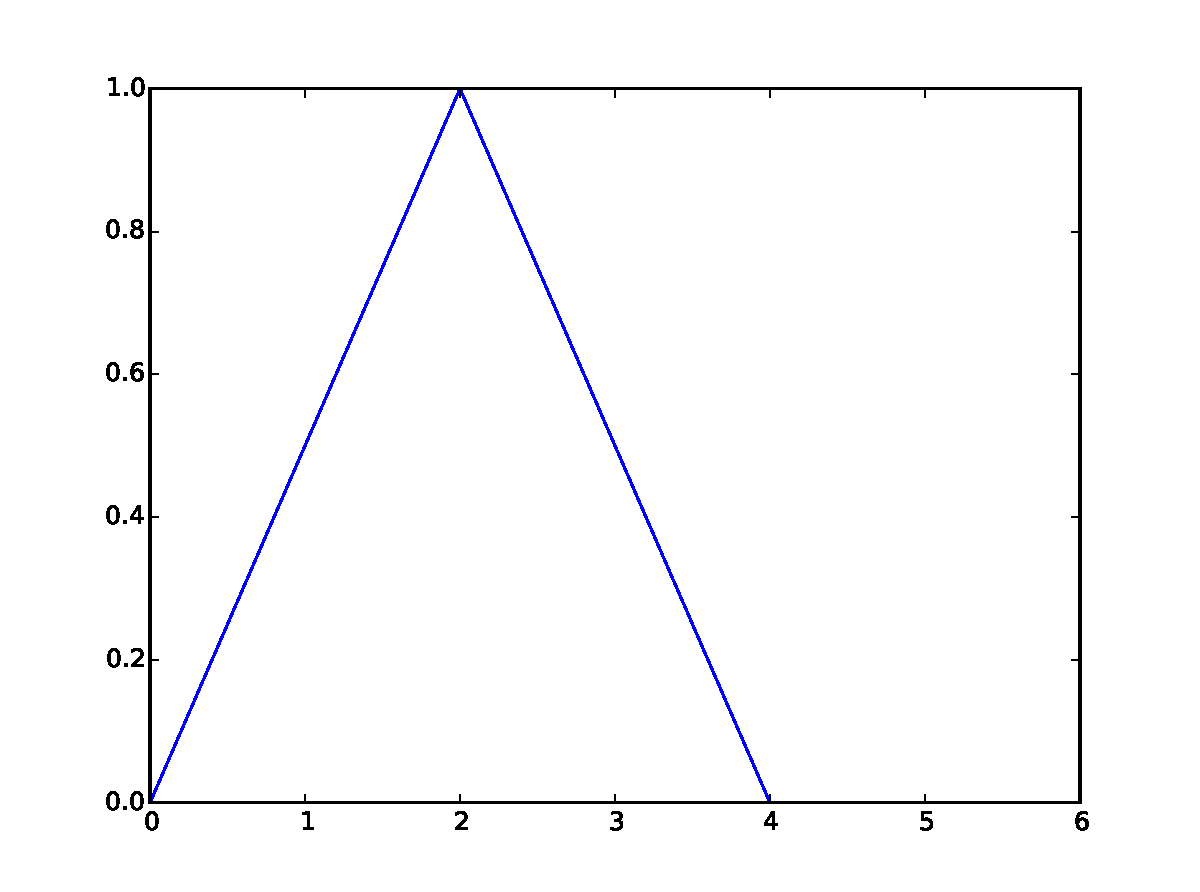
\includegraphics[width=\textwidth]{basis_2.pdf}
\end{subfigure}
\caption{basis function for single variable scenarios}\label{basisSingle}
\end{figure}
Let $\xi$ be the uncertain demand $\in [l,u]$ and $\{x_{i},0 \leq i \leq n:x_0 =l,x_n= u\}$ be breakpoints. Define
$$
L_0(\xi) = \left\{
\begin{array}{ll}
1-(\xi-l)/(x_1-l) & \xi \in [l,x_1]\\
0 & \xi \in (x_1,u]
\end{array}
\right.
$$
$$
L_1(\xi) = \left\{
\begin{array}{ll}
(\xi-l)/(x_1-l) & \xi \in [l,x_1]\\
1-(\xi-x_1)/(x_2-x_1) & \xi \in (x_1,x_2]\\
0 & \xi \in (x_2,u]
\end{array}
\right.
$$
 as shown in figure \ref{basisSingle} and so on. Actually, we have
$$
L_i(\xi) = \left\{
\begin{array}{ll}
0 & \xi\in[0,x_{i-1}]\\
(\xi-x_{i-1})/(x_i-x_{i-1}) & \xi \in (x_{i-1},x_i]\\
1-(\xi-x_i)/(x_{i+1}-x_i) & \xi \in (x_i,x_{i+1}]\\
0 & \xi \in (x_{i+1},u]
\end{array}
\right.
$$
for $0\leq i \leq n$.Define lifting operator
$$
L(\xi) =
\left(
\begin{array}{c}
L_0(\xi)\\
L_1(\xi)\\
\ldots\\
L_n(\xi)
\end{array}
\right)
$$
It is not hard to get corresponding retraction operator
$$
R\circ L (\xi) = \sum\limits_{i=0}^n x_i L_i(\xi) = \xi
$$
If we are going to solve original problem following where $\mathbf{\xi},\mathbf{c(\xi)}$ and $\mathbf{x(\xi)}$ are all vectors.
$$
\begin{array}{ll}
\min & \mathbb{E_\xi}\mathbf{c}^T \mathbf{x(\xi)}\\
s.t. & Z(\mathbf{x(\xi)}) \geq 0 \\
& \forall \xi \in \Xi \{(\xi_i)_{len}:l_i \leq \xi_i \leq u_i \}
\end{array}
$$
We have to consider about defining $L$ again,that is
$$L^i(\xi) =
\left(
\begin{array}{c}
L_0(\xi_i)\\
L_1(\xi_i)\\
\ldots\\
L_n(\xi_i)
\end{array}
\right)$$
and
$$
\tilde{L}(\xi) =
\left(
\begin{array}{c}
L^1(\xi)\\
L^2(\xi)\\
\ldots\\
L^{len}(\xi)
\end{array}
\right)
$$
$$
\tilde{R}\circ \tilde L (\xi) =
\left(
\begin{array}{c}
R^1(L^1(\xi))\\
R^2(L^2(\xi))\\
\ldots\\
R^{len}(L^{len}(\xi))
\end{array}
\right)
$$
Approaching the original problem with lifting variables, we will have below equation
$$
\begin{array}{ll}
\min & \mathbb{E}_{R(\xi)}  \mathbf{c}^T X\xi\\
s.t. & ZX\xi \geq 0 \\
& \forall \xi \in \tilde{L}(\Xi)
\end{array}
$$
And actually $\tilde{R}(\cdot)$ could be replaced by a matrix $\hat{R}$. Now we are going to discuss about $L(\Xi)$.As we want to utilize duality arguments, so we need to replace $\tilde{L}(\Xi)$ with $conv \tilde{L}(\Xi)$. It could be no better if we don't have to add more constraints in LP during lifting.As we all know,
$$conv\tilde{L}(\Xi) = \prod\limits_{i=1}^{len} conv L^i(\Xi) $$
So we only need to care about singe variable lifting $L^i(\xi) = L(\xi_i)$ again. That is why I call it single variable scenarios.For the sake of simplicity synonym, I will omit index $i$ on both $L^i(\cdot)$ and $\xi_i$ now.As for $conv L(\xi)$,actually we have
$$
conv L(\Xi) = conv\{\mathbf{e_0},\cdots,\mathbf{e_n}\}
$$
where $\{\mathbf{e_i}\}$ are standard basis in euclidian space.
It is because that for any realisation $\xi \in \Xi$, at most two elements of $\xi$ are non-zero. Let $i$th and $i+1$th element be the non-zero. Benefiting from piecewise linear basis functions, in fact, we have
$$\xi = \xi_i \mathbf{e_i} + \xi_{i+1} \mathbf{e_{i+1}}$$
$$\xi_i+\xi_{i+1}=1,\xi_i\geq0,\xi_{i+1}\geq 0$$
Therefore,
$$
conv L(\Xi)  \subseteq conv\{\mathbf{e_0},\cdots,\mathbf{e_n}\}
$$
In the meantime, $$\{\mathbf{e_0},\cdots,\mathbf{e_n}\} \subseteq conv L(\Xi)$$
So we can tell that
$$
conv L(\Xi) = conv\{\mathbf{e_0},\cdots,\mathbf{e_n}\}
$$
What's more,as $conv\{\mathbf{e_0},\cdots,\mathbf{e_n}\}$ are corner points of the feasible region, we can keep constraints unchanged.
\section{Multivariate Scenarios}
\begin{figure}
\centering
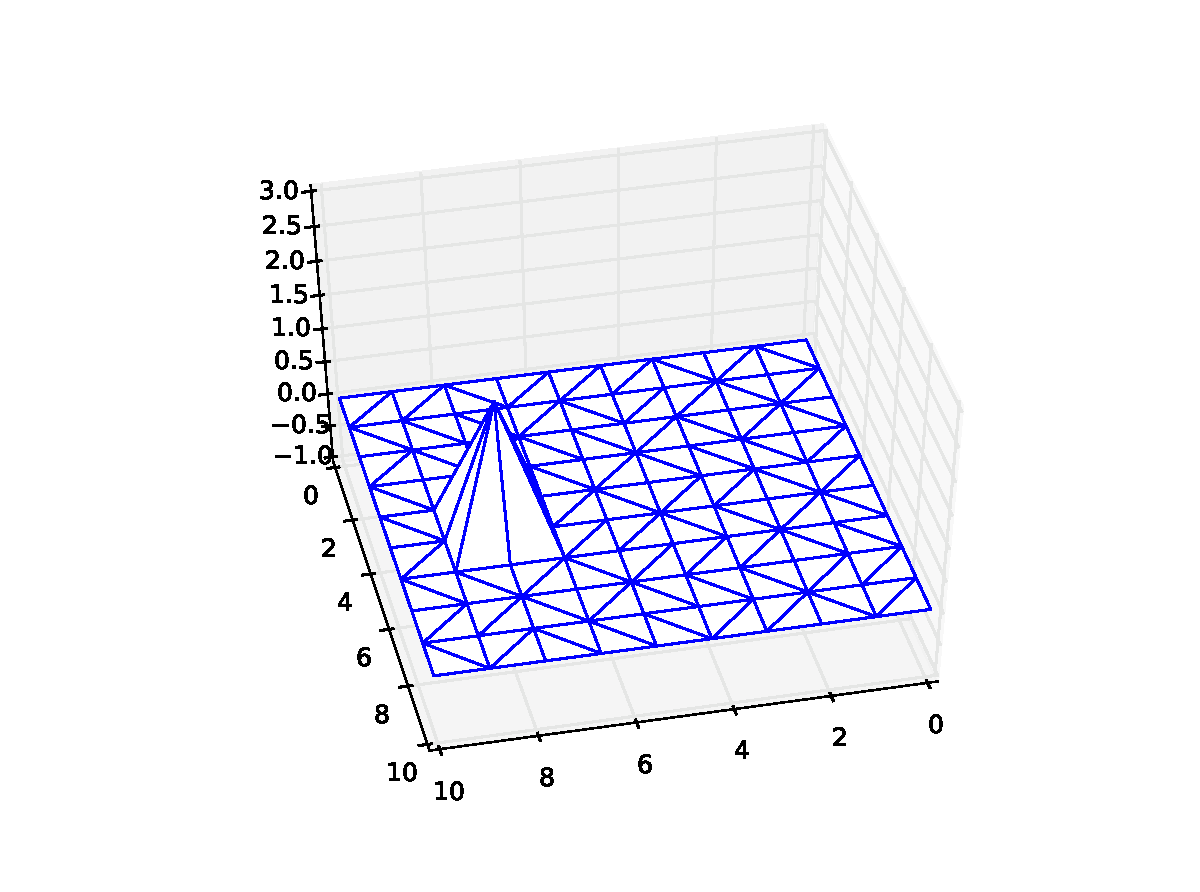
\includegraphics[width=\textwidth]{basis_3.pdf}
\caption{basis functions for multivariate scenarios}\label{multi}
\end{figure}
Same as single variable scenarios, let $(\xi,\eta)$ still be the uncertain demand,but now we have to do triangulation on 2-d mesh grid. Let $\{(x_m,y_m),0 \leq m \leq n\} $ be points on triangular meshs. As shown in figure \ref{multi}, piecewise linear function $L_i(\xi,\eta)$ now is defined by
$$
L_i(x_i,y_i) = 1
$$
$$
L_i(\hat{x},\hat{y}) = 0 ,\forall (\hat{x},\hat{y}) \in \{(x_m,y_m),0 \leq m \leq n\}\backslash \{(x_i,y_i)\}
$$
Also, we can define
$$
L(\xi,\eta) =
\left(
\begin{array}{c}
L_0(\xi,\eta)\\
L_1(\xi,\eta)\\
\ldots\\
L_n(\xi,\eta)
\end{array}
\right)
$$
with retraction operator 
$$
R\circ L(\xi,\eta) = \sum\limits_{i=0}^{n} (x_i,y_i) L_i(\xi,\eta) = (\xi,\eta)
$$
Now consider about applying it on
$$
\begin{array}{ll}
\min & \mathbb{E_\xi}\mathbf{c}^T \mathbf{x(\xi)}\\
s.t. & Z(\mathbf{x(\xi)}) \geq 0 \\
& \forall \xi \in \Xi \{(\xi_i)_{len}:l_i \leq \xi_i \leq u_i \}
\end{array}
$$
If we are attempting to approach with $x(\sum\limits_{i=1}^{t-1}\xi_i,\xi_t)$.We should design lifting demands like
$$
\tilde{\xi}=(\xi_1,\xi_2,\cdots,\xi_T,L(\xi_1,\xi_2),L(\xi_1+\xi_2,\xi_3),\cdots,L(\sum\limits_{i=1}^{T-1}\xi_i,\xi_T))^T
$$
that is
$$
\begin{array}{ll}
\tilde{\xi} \in \Xi' =& \{(\xi'_1,\xi'_2,\cdots,\xi'_T,\xi'_{T+1},\xi'_{T+2},\cdots,\xi'_{T+T-1})^T:l_i\leq \xi'_i \leq u_i,1\leq i \leq T,\\
&L(\sum\limits_{i=1}^t \xi'_i,\xi'_{t+1}) = \xi'_{T+t}, 1\leq t\leq T-1\}
\end{array}
$$
The left problem is how to get $conv\Xi'$.In fact,
$$
\begin{array}{ll}
\Xi' = &\{(\xi_1',\xi_2',\cdots,\xi'_T,\xi'_{T+1},\xi'_{T+2},\cdots,\xi'_{T+T-1})^T:l_i\leq \xi'_i \leq u_i,1\leq i \leq T,\\
&\xi'_{T+t}\in \bigcup\limits_{i,j,k} conv\{\mathbf{e_i},\mathbf{e_j},\mathbf{e_k}\}\text{($i,j,k$ are neighbourhood points)},\\
& \sum\limits_{i=1}^t \xi'_i = (R(\xi'_{T+t}))_1,\xi_{t+1} = (R(\xi'_{T+t}))_2, 1\leq t\leq T-1 \}
\end{array}
$$
Let 
$$
\begin{array}{ll}
A = &\{(\xi_1',\xi_2',\cdots,\xi'_T,\xi'_{T+1},\xi'_{T+2},\cdots,\xi'_{T+T-1})^T:l_i\leq \xi'_i \leq u_i,1\leq i \leq T,\\
&\xi'_{T+t}\in \bigcup\limits_{i,j,k} conv\{\mathbf{e_i},\mathbf{e_j},\mathbf{e_k}\}\text{($i,j,k$ are neighbourhood points)},1\leq t\leq T-1\}\\
\end{array}
$$
$$
\begin{array}{ll}
B = &\{(\xi_1',\xi_2',\cdots,\xi'_T,\xi'_{T+1},\xi'_{T+2},\cdots,\xi'_{T+T-1})^T:l_i\leq \xi'_i \leq u_i,1\leq i \leq T,\\
& \sum\limits_{i=1}^t \xi'_i = (R(\xi'_{T+t}))_1,\xi_{t+1} = (R(\xi'_{T+t}))_2, 1\leq t\leq T-1 \}
\end{array}
$$
We have $conv(A\bigcap B)$ = $convA \bigcap B$
\begin{proof}
Assuming it is false, there will be a element $\xi$ in $convA \bigcap B$ but not in $conv(A\bigcap B)$. As $\xi \in convA$, so we can let $\xi = \lambda_1 \xi_1+\lambda_2 \xi_2 (\lambda_1\geq0,\lambda_2> 0,\lambda_1+\lambda_2 \leq 1)$,where $\xi_1 \in A\bigcap B$  and $\xi_2 \in A\backslash(A\bigcap B)$. But as we can see, the constraints in B is linear. So $\xi$ mustn't belong to B otherwise $\xi_2 = (\xi-\lambda_1 \xi_1)/\lambda_2 \in B$.
\end{proof}
In other words, we have
$$
\begin{array}{ll}
conv\Xi' = &conv\{(\xi_1',\xi_2',\cdots,\xi'_T,\xi'_{T+1},\xi'_{T+2},\cdots,\xi'_{T+T-1})^T:l_i\leq \xi'_i \leq u_i,1\leq i \leq T,\\
&\xi'_{T+t}\in \bigcup\limits_{i,j,k} conv\{\mathbf{e_i},\mathbf{e_j},\mathbf{e_k}\}\text{($i,j,k$ are neighbourhood points)},1\leq t\leq T-1\}\\
&\bigcap\{(\xi_1',\xi_2',\cdots,\xi'_T,\xi'_{T+1},\xi'_{T+2},\cdots,\xi'_{T+T-1})^T:l_i\leq \xi'_i \leq u_i,1\leq i \leq T,\\
&\sum\limits_{i=1}^t \xi'_i = (R(\xi'_{T+t}))_1,\xi_{t+1} = (R(\xi'_{T+t}))_2, 1\leq t\leq T-1 \}\\
& = \{(\xi_1',\xi_2',\cdots,\xi'_T,\xi'_{T+1},\xi'_{T+2},\cdots,\xi'_{T+T-1})^T:l_i\leq \xi'_i \leq u_i,1\leq i \leq T,\\
&\xi'_{T+t}\in conv\{\mathbf{e_0},\mathbf{e_1},\cdots,\mathbf{e_n}\},\sum\limits_{i=1}^t \xi'_i = (R(\xi'_{T+t}))_1,\xi_{t+1} = (R(\xi'_{T+t}))_2, 1\leq t\leq T-1 \}\\
\end{array}
$$
Therefore, we won't change constraints in the end.
Also,it is possible for us to approach original problem with $x(\max\{\xi_1,\xi_2,\cdots,\xi_{t-1}\},\xi_t)$.
\end{document}
